\documentclass[xcolor=dvipsnames,12pt]{beamer} %pt10,11,12
\usefonttheme{serif}
\usepackage{graphicx}
\usepackage{subfigure}
\usepackage{multicol}
\usepackage[figurename=]{caption}
%%\usepackage{xcolor}
\usepackage{hyperref}
\hypersetup{
    colorlinks=true,%
    citecolor=blue,%
    filecolor=black,%
    linkcolor=blue,%
    urlcolor=blue
}


\setlength{\parskip}{2ex}

\title{Using Latent Variable Models to Estimate the Prevalence of Sexual Violence in Armed Conflict: An Introduction}
\author{Jule Kr\"{u}ger, \\ Center for Political Studies, University of Michigan\\[.5cm]
\emph{Workshop on Empirical and Computational Social Sciences in India}\\[.5cm] Ashoka University, December 15, 2018}
\date{}
\begin{document}

\frame{\titlepage}

\frame{
This tutorial builds on ongoing research with

\begin{multicols}{2}

\begin{figure}
\includegraphics[width=4cm]{hand/RNordaas.jpeg}\caption{\href{https://ragnhildnordas.wordpress.com/}{Ragnhild Nord\r{a}s}}
\end{figure}
and 
\begin{figure}
\includegraphics[width=5cm]{hand/CFariss.jpg}\caption{\href{http://cfariss.com/}{Christopher Fariss}}
\end{figure}
\end{multicols}

}

\frame{\frametitle{Outline}

\begin{enumerate}
\item Wartime sexual violence and observational dynamics
\item Observed levels of conflict-related sexual violence
\item A broad overview of the latent variable model (LVM) 
\item Estimating LVM in R and visualizing different model outcomes
\item A dynamic specification
\item Outlook
\end{enumerate}
}

\frame{\frametitle{Wartime Sexual Violence}%\pause

\begin{itemize}
\item Includes the use of rape and other forms of sexual violence
\item Constitutes a severe human rights problem
\item Is difficult to observe and document as a practice
\end{itemize}

A lack of systematic data impedes empirical analysis with regard to extent, spatiotemporal trends, and patterns.

}

\frame{\frametitle{Why Conflict-Related Sexual Violence  Is Hard to Measure}%\pause
\begin{itemize}
\item Shame, fear of retaliation, stigma and rejection due to socio-cultural taboos
\item Inconsistency in testimony and lack of clear narrative due to trauma-induced memory loss
\item Differing conceptualizations and language  used to refer to sexual violence events
\item Perpetrators' incentives to conceal activity and evade accountability for war crimes
\item Blending of state actors and institutions with regard to the perpetration and reporting of these crimes

\end{itemize}

All of these issues vary over space and time.

}

\frame{\frametitle{Why the Observation of Wartime Sexual Violence May Change over Time}%\pause

\begin{itemize}
\item Increasing international focus
\item Changing norms and perceptions of survivors
\item Recent challenges to societal taboos
\item Growing initiatives to empower survivors to speak out
\item Changes in the wording of sexual violence experiences leading to more explicit descriptions
\item Growth in documentation efforts paired with improved documentation practices
\end{itemize}

While these trends  vary across space, we will likely see higher reporting rates in some places  over time.

}

\frame{\frametitle{How We Currently Measure Wartime Sexual Violence}

\begin{figure}
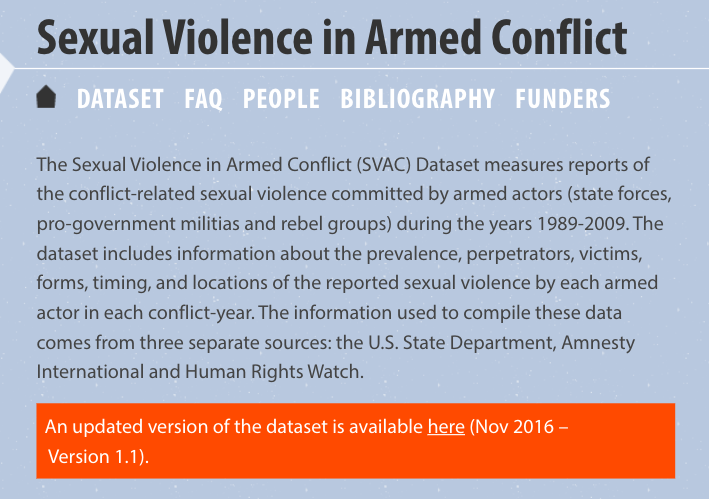
\includegraphics[width=8.5cm]{hand/SVAC-home.png}
\caption{Three ordinal SVAC variables based on human-coded annual human rights reports \url{http://www.sexualviolencedata.org/}}
\end{figure}
}

\frame{Let's import the data into R and take a look at it:

\begin{itemize}
\item[{\tt \$:}] {\tt cd \textasciitilde/git/SVAC-LVM-tutorial/import}
\item[{\tt \$:}]  {\tt open -a Rstudio src/import-check-data-main.R}
\end{itemize}

In this tutorial, we will only look at reported SVAC with respect  to state forces (`GOV').

}

\begin{frame}[label=SUDAN-obs]
\frametitle{SVAC Provides Three Indicators that Report Prevalence of Wartime Sexual Violence: Sudan}
\begin{figure}\centering
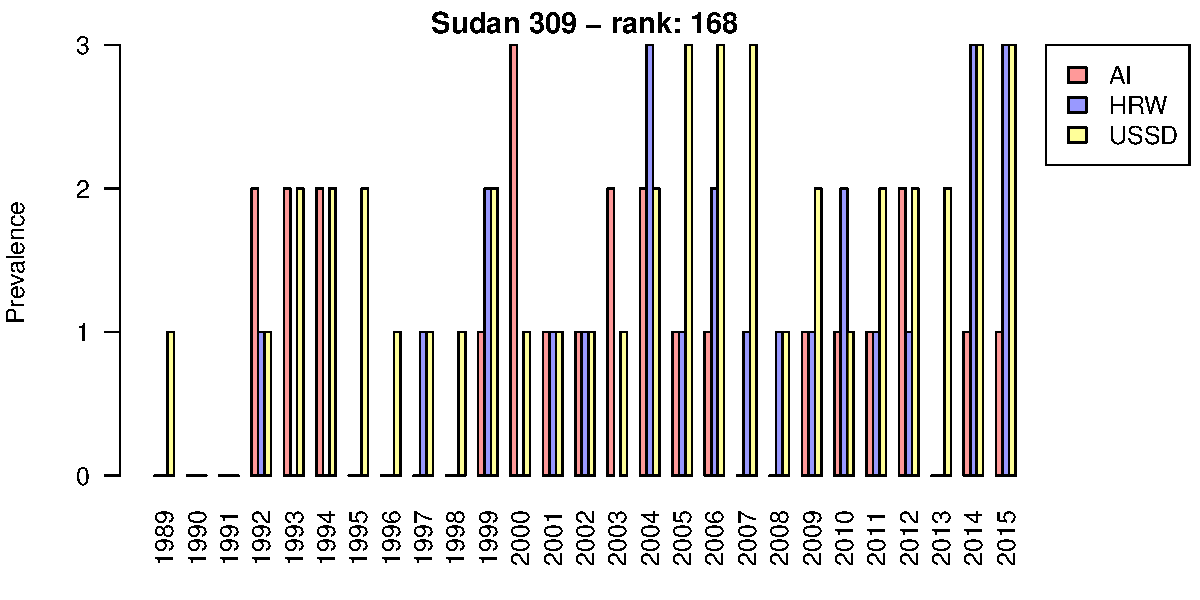
\includegraphics[width=11cm]{../visualize/output/bp-obs-GOV-Sudan-309.pdf}
\caption{Reported level of engagement in wartime sexual violence by state forces in Sudan according to three sources \hyperlink{SUDAN-static}{\beamerbutton{static}}}
\end{figure}
\end{frame}


\begin{frame}[label=DRC-obs]
\frametitle{Another Case: DRC }
\begin{figure}\centering
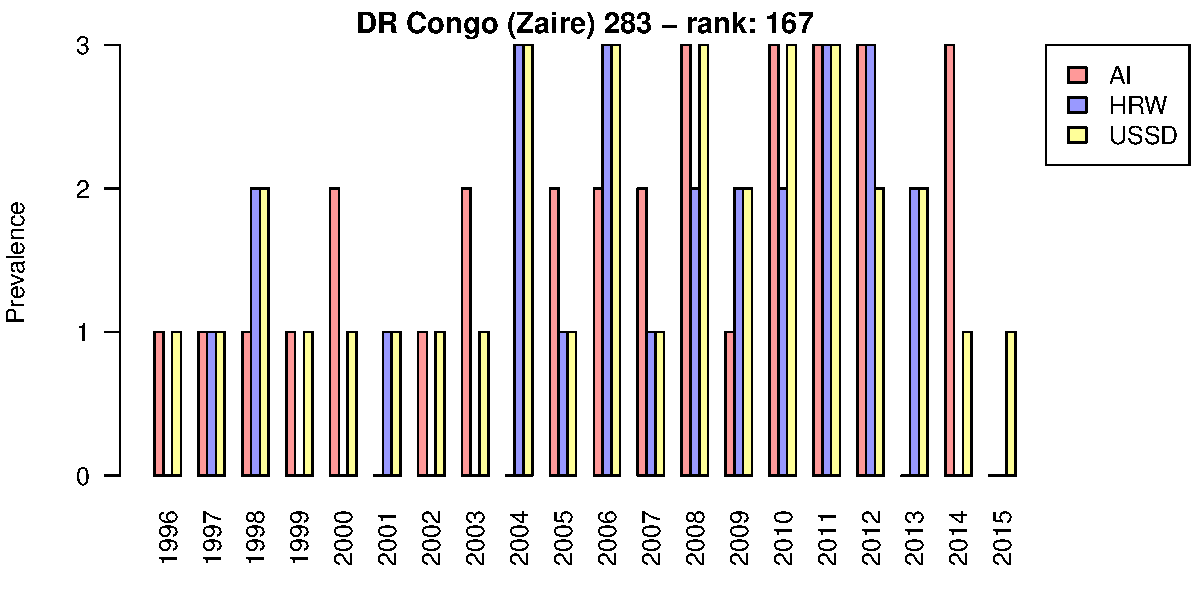
\includegraphics[width=11cm]{../visualize/output/bp-obs-GOV-DR-Congo-Zaire-283.pdf}
\caption{Reported level of engagement in wartime sexual violence by state forces in DRC according to three sources \hyperlink{DRC-static}{\beamerbutton{static}}}
\end{figure}
\end{frame}

% \frame{
% 
% Let's make some more barplots of reported state behavior for other armed conflict cases:
% 
% \begin{itemize}
% \item[{\tt \$:}] {\tt cd ../visualize}
% \item[{\tt \$:}] {\tt open -a Rstudio  src/barplot-sources-by-conflict.R}
% \end{itemize}
% 
% }

\frame{\frametitle{For Every Conflict-Year, We Have Three Sources Reporting on SVAC Prevalence}
\begin{itemize}
\item For many years, the three prevalence measures diverge (e.g., Sudan 2006, DRC 1998)
\item In other years, the three sources seem to agree (e.g., Sudan 2001-2, DRC 2011)
\item In a considerable number of  years (when looking at the entire dataset), the three sources do not report any SV (e.g., Sudan 1990-1) 
\end{itemize}

How do we deal with converging/diverging information across the three sources? Shall we average across them, or should we choose the ``best''/most common/lowest/highest level?

}

\frame{\frametitle{What If, for a Given Conflict-Year, We Understand}


\begin{itemize}
\item True SVAC prevalence as a \emph{latent trait} that can't be observed directly but estimated using observed outcomes
\item Available human rights reports  as imperfect measures of the latent level  due to observational challenges
\item Human-coded SVAC variables as imperfect measures of human rights reports due to perceptual coding error
\item Information convergence/divergence across sources as a measure of certainty regarding SVAC prevalence
\end{itemize}

The logic of latent variable models (LVM) follows precisely this conceptual approach to measurement. 
}

\frame{\frametitle{The Added Value of Latent Variable Models}

\begin{itemize}
\item Leverage information from multiple sources
\item Average across them while accounting for their respective measurement error
\item Provide probabilistic estimates of a latent trait,  SVAC in our case 
\item Express  our  uncertainty  regarding the estimates of the latent trait through credible intervals 
\item Compute the estimated latent trait at the interval-level (instead of ordinal), which simplifies subsequent analysis 
\item Enable direct probabilistic comparisons across conflict-years and cases
\end{itemize}

}

\frame{\frametitle{Parametrizing a LVM to Estimate SVAC, I}

(Cf.\ \href{http://cfariss.com/documents/SchnakenbergFariss2014PSRM.pdf}{Schnakenberg and Fariss (2014:7-10)} for details.)

We assume that the observed human rights reports for each conflict-year are functions of a unidimensional latent variable $\theta$ that represents the level of SVAC.

For each conflict-year observation, we index conflicts with $i$ and years with $t$.

For each model, we have three ordinal indicators $J$ with levels 0 (no reports), 1 (some), 2 (several/many), and 3 (massive). 

}

\frame{\frametitle{Parametrizing a LVM to Estimate SVAC, II}

The observed values of each indicator (or, ``item'') are denoted as $y_{itj}$ for a given conflict-year and assumed to depend on $\theta_{it}$.

Using these observed values, our goal is to estimate $\theta_{it}$, i.e., the latent SVAC prevalence in conflict $i$ in year $t$.

For each item (i.e., indicator), we estimate an ``item discrimination'' parameter $\beta_{j}$ and a set of $K_{j}-1$ difficulty cut-points $(\alpha_{jk})^{k_{j}}_{k=1}$. (We will plot these cut-points later on.)

}

\frame{\frametitle{Parametrizing a LVM to Estimate SVAC, III}

There is also an error term $\varepsilon_{itj}$ for each item, which in our case represents observational challenges and coding errors. 

We assume that the error terms are independently drawn from a logistic distribution.

The distribution of the error terms determines the likelihood of our model.

}

\frame{\frametitle{Estimating a Latent Variable Model}

Following our parametrization, we can derive a probability distribution for a given response  to item $j$.

A likelihood function for $\beta$, $\alpha$ and $\theta$ given the data enables estimation of our unobserved parameters.

If you are interested in the math underlying Bayesian ordinal item-response theory, please refer to Schnakenberg and Fariss (2014: 7-8) for a start. 

For time constraints, we will limit our tutorial to LVM implementation in R.

}


\frame{\frametitle{Let's Run Some LVMs.}

\begin{itemize}
\item[{\tt \$:}] {\tt cd ../estimate}
\item[{\tt \$:}] {\tt open -a Rstudio  src/estimate-static-SVAC.R}
\end{itemize}
}

\frame{\frametitle{Checking Model Convergence}

We can check whether our model converged successfully by plotting the Rhat statistic. 

If the Rhat values remain below 1.1, we conclude model convergence has occurred.

If the values are above 1.1, we would rerun the model with a higher number of iterations until we reach convergence.
}

\frame{\frametitle{An Rhat Plot for the Static LVM}


\begin{figure}\centering
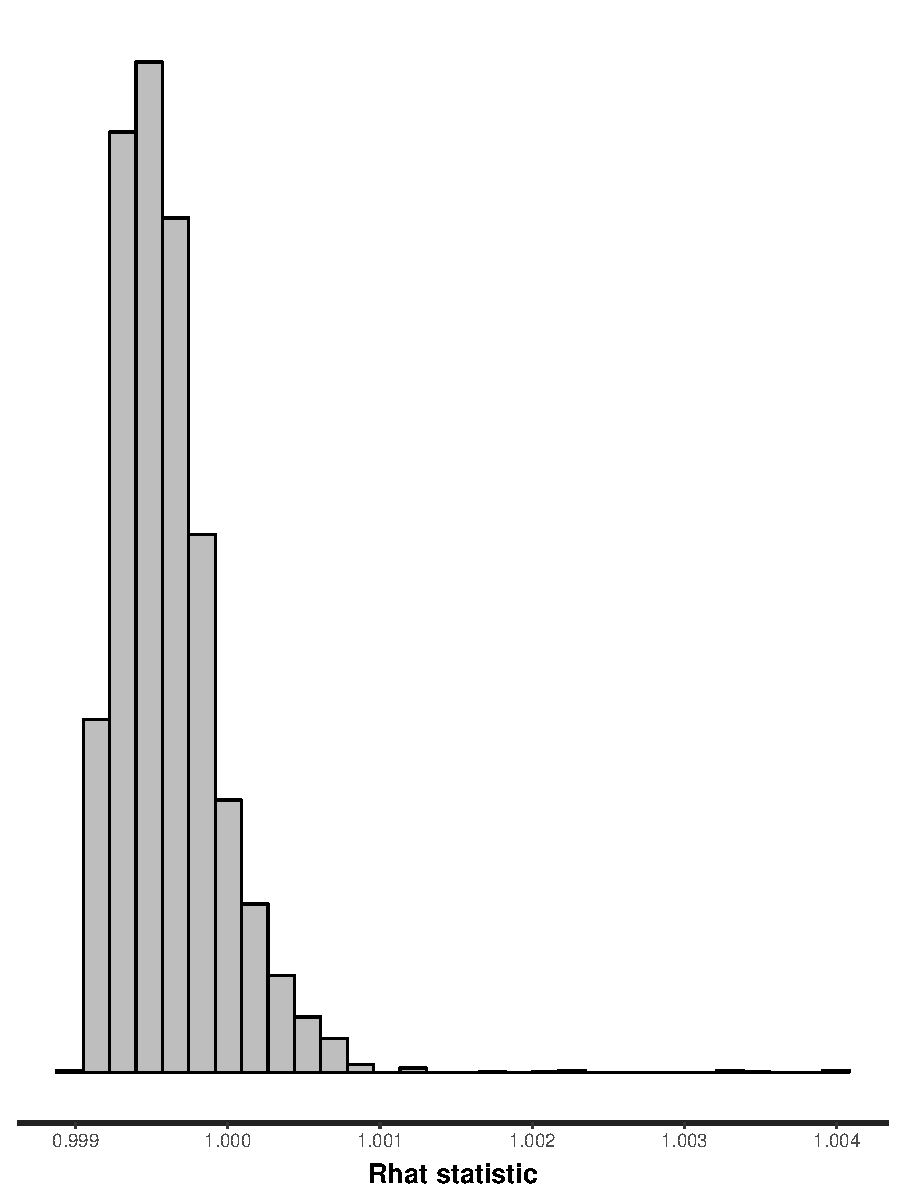
\includegraphics[width=6cm]{../estimate/output/gg-rhat-SVAC-static.pdf}
%\caption{ This looks good! }
\end{figure}

}

\frame{\frametitle{Plotting the $\alpha$ Difficulty Cut-Points}

%% The high cutpoints are to be expected because most of the latent variable mass is at 0. 
%% These cut points push up just a small number of units. 

\begin{figure}
\subfigure[AI]{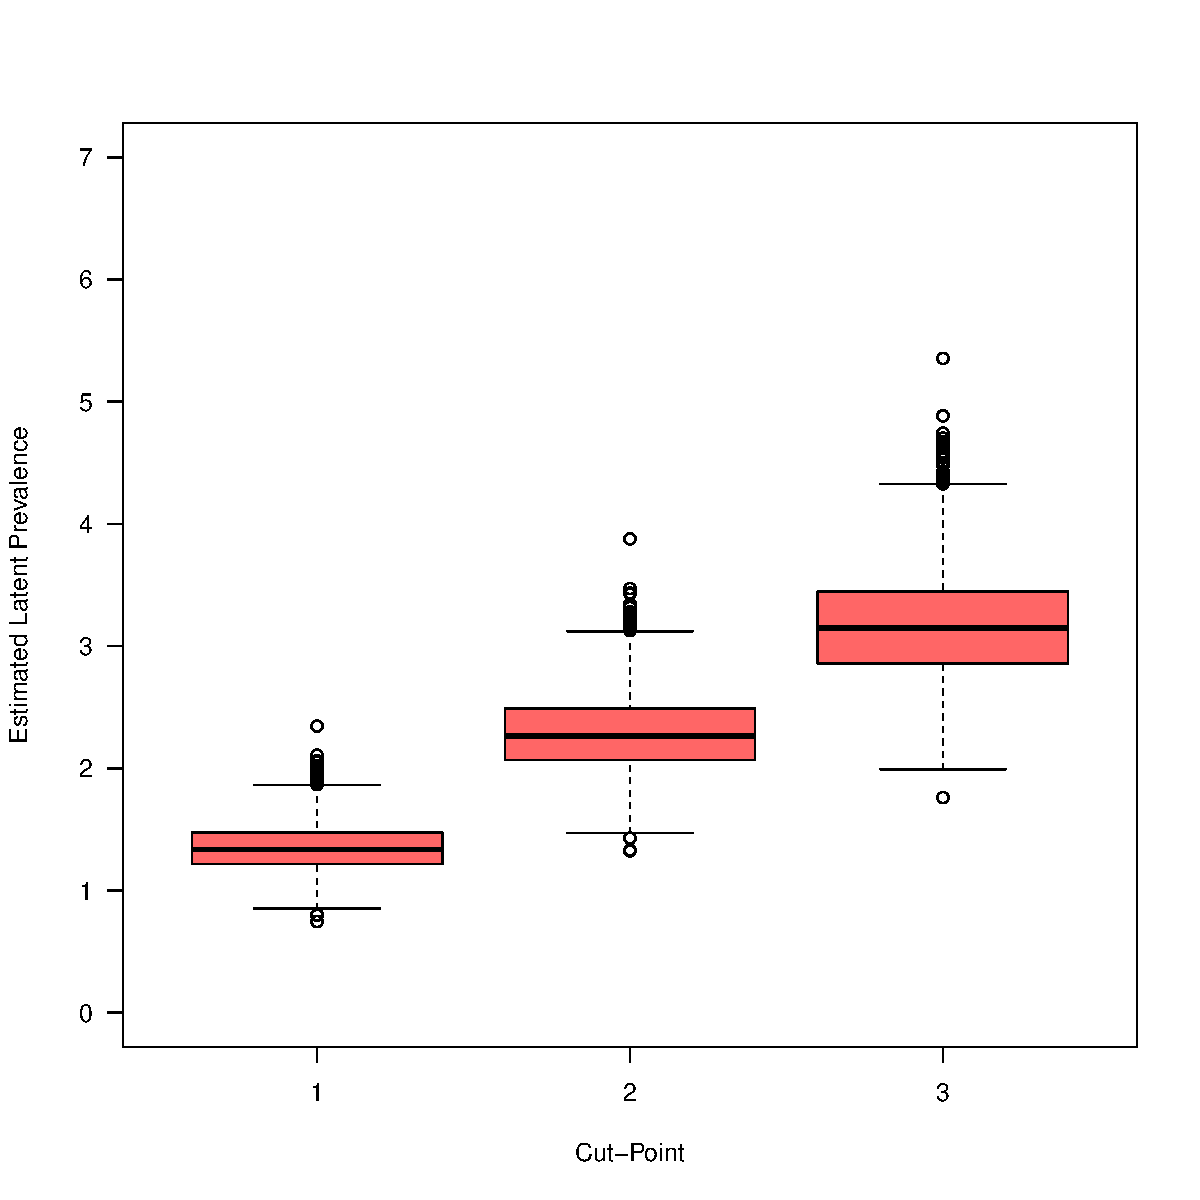
\includegraphics[width=3.5cm]{../estimate/output/bp-cp-static-ai.pdf}}
\subfigure[HRW]{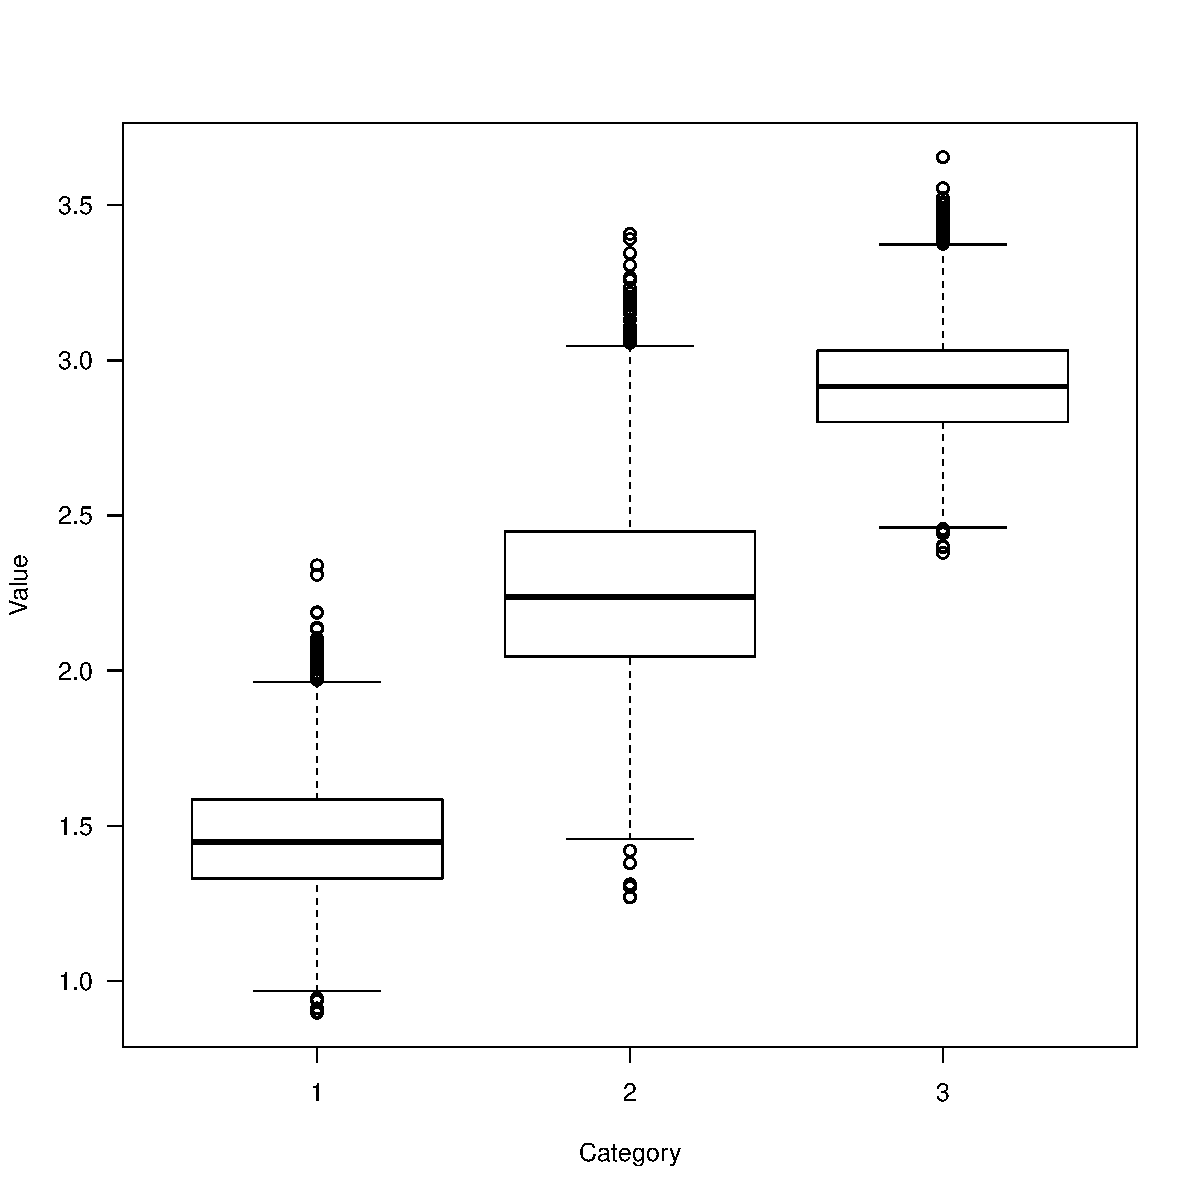
\includegraphics[width=3.5cm]{../estimate/output/bp-cp-static-hrw.pdf}}
\subfigure[USSD]{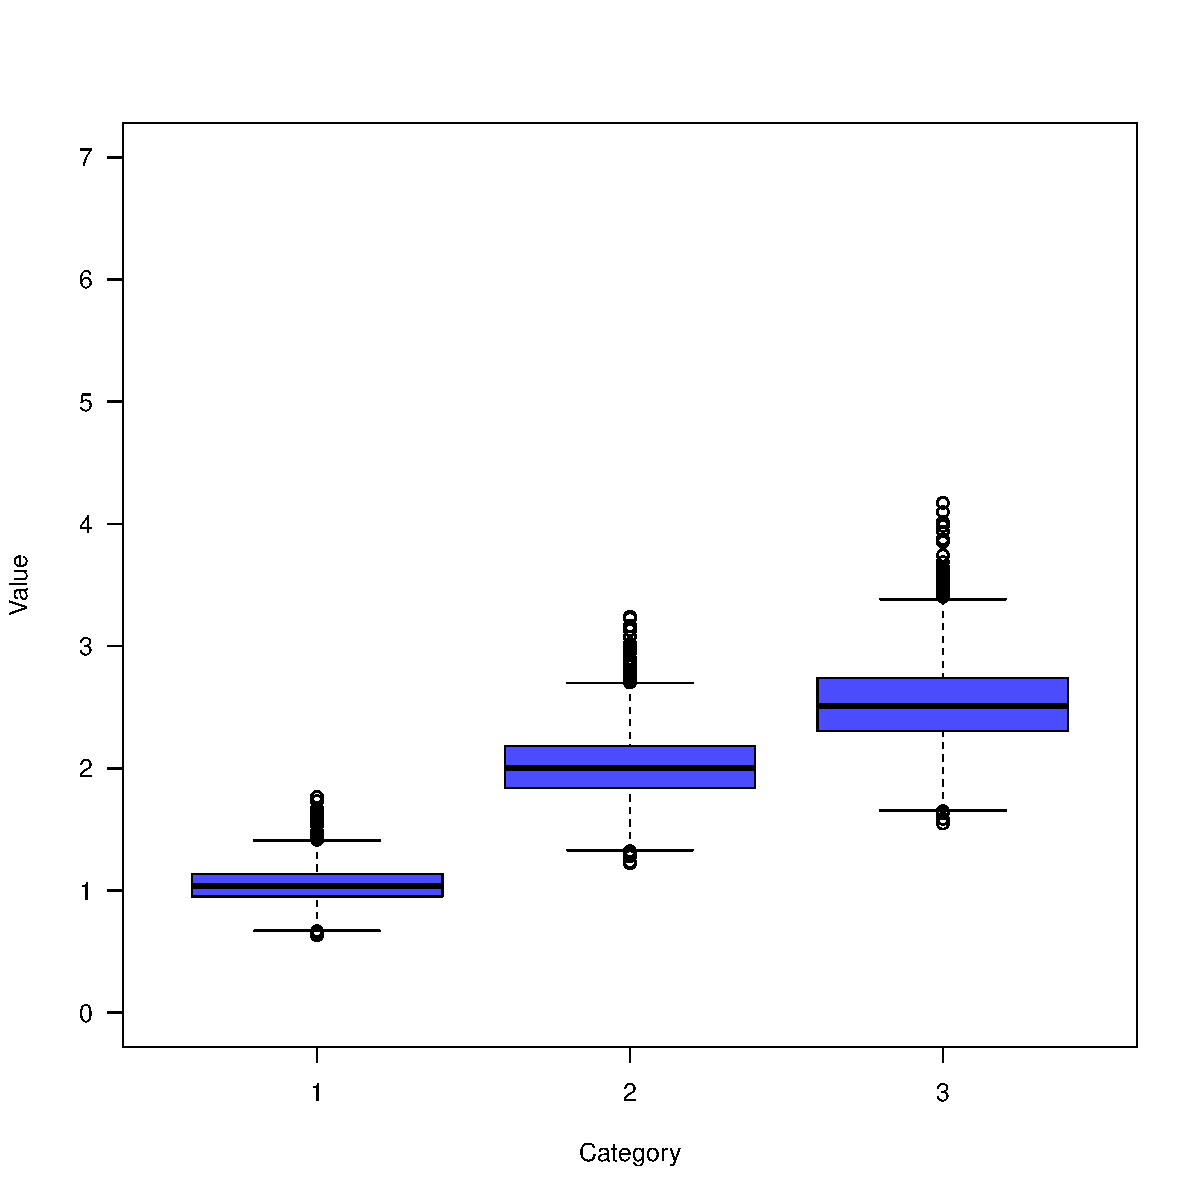
\includegraphics[width=3.5cm]{../estimate/output/bp-cp-static-state.pdf}}
\end{figure}
}

\frame{\frametitle{Visualizing Our $\theta$ Estimates}

\begin{itemize}
\item[{\tt \$:}] {\tt cd ../visualize}
\item[{\tt \$:}] {\tt open -a Rstudio  src/plot-LVM-estimates-by-conflict.R}
\end{itemize}
}

\begin{frame}[label=SUDAN-static]
\frametitle{Static Estimates of the Latent Prevalence of Wartime Sexual Violence: Sudan}
\begin{figure}\centering
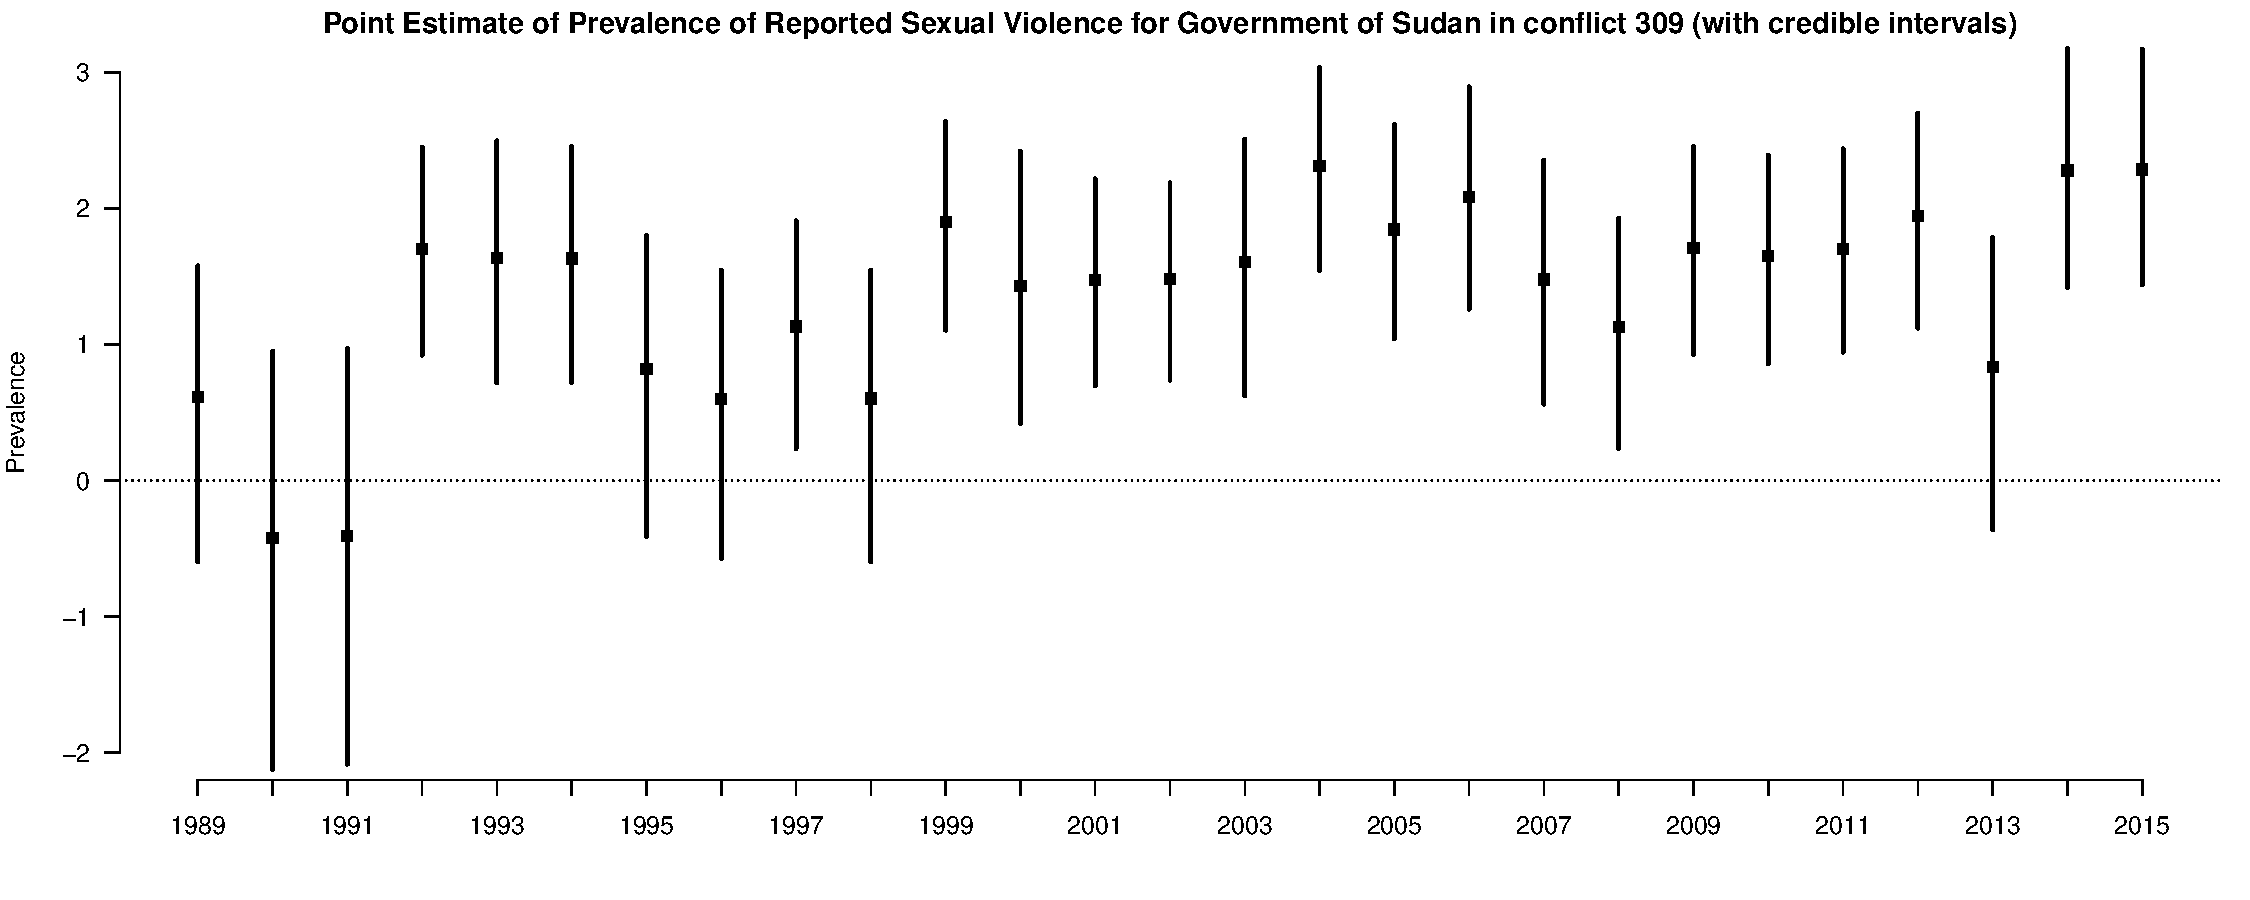
\includegraphics[width=11cm]{../visualize/output/pp-static-estimates-Sudan-309.pdf}
\caption{Estimated level of engagement in wartime sexual violence by state forces in Sudan \hyperlink{SUDAN-obs}{\beamerbutton{obs}}\hyperlink{SUDAN-dynamic}{\beamerbutton{dynamic}}}
\end{figure}
\end{frame}


\begin{frame}[label=DRC-static]
\frametitle{Static Estimates: DRC}
\begin{figure}\centering
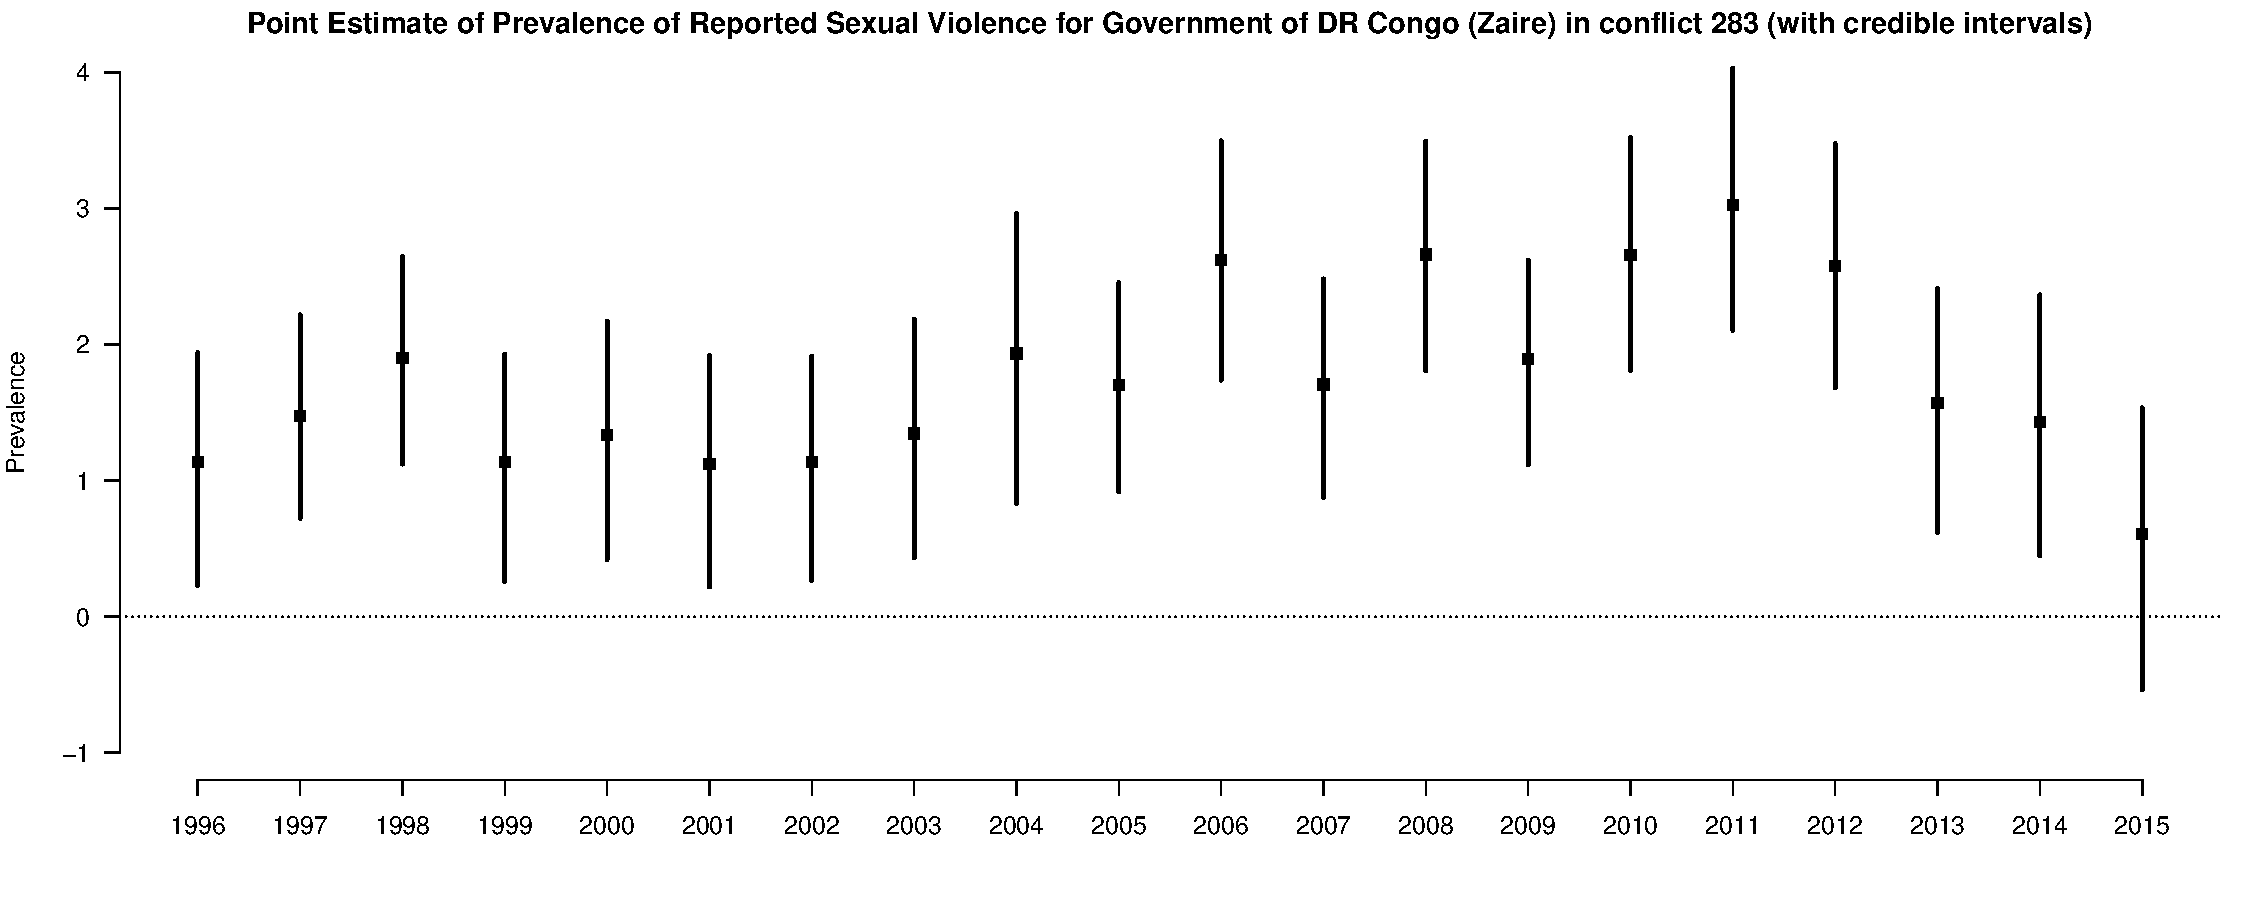
\includegraphics[width=11cm]{../visualize/output/pp-static-estimates-DR-Congo-Zaire-283.pdf}
\caption{Estimated level of engagement in wartime sexual violence by state forces in DRC \hyperlink{DRC-obs}{\beamerbutton{obs}}\hyperlink{DRC-dynamic}{\beamerbutton{dynamic}}}
\end{figure}
\end{frame}

\frame{\frametitle{The Local Independence Assumption in a Static Model}

Item-Response Theory requires us to assume local independence in LVMs:

\begin{itemize}
\item[(1)] local independence of different indicators within the same conflict-year,
\item[(2)] local independence of indicators across conflicts within years,
\item[(3)] local independence of indicators across years within countries.
\end{itemize}

In the static model, we place independent standard normal prior on each $\theta_{it}$.
}

\frame{\frametitle{Relaxing the (3) Local Independence Assumption in a Dynamic Model}

We relax the (3) local independence assumption to estimate a dynamic model.

\begin{itemize}
\item Empirical conflict research shows that the level of  political violence in a given year often depends on the level of political violence in the previous year.
\item It is similarily plausible that observational challenges are time-dependent in this way.
\end{itemize}

In a dynamic model, we specify hierarchical priors for each $\theta_{it}$ that allow the estimated latent level of wartime sexual violence in a given conflict-year to depend on that conflict's value in the previous year.
}

\begin{frame}[label=SUDAN-dynamic]
\frametitle{Dynamic Estimates of the Latent Prevalence of Wartime Sexual Violence: Sudan}
\begin{figure}\centering
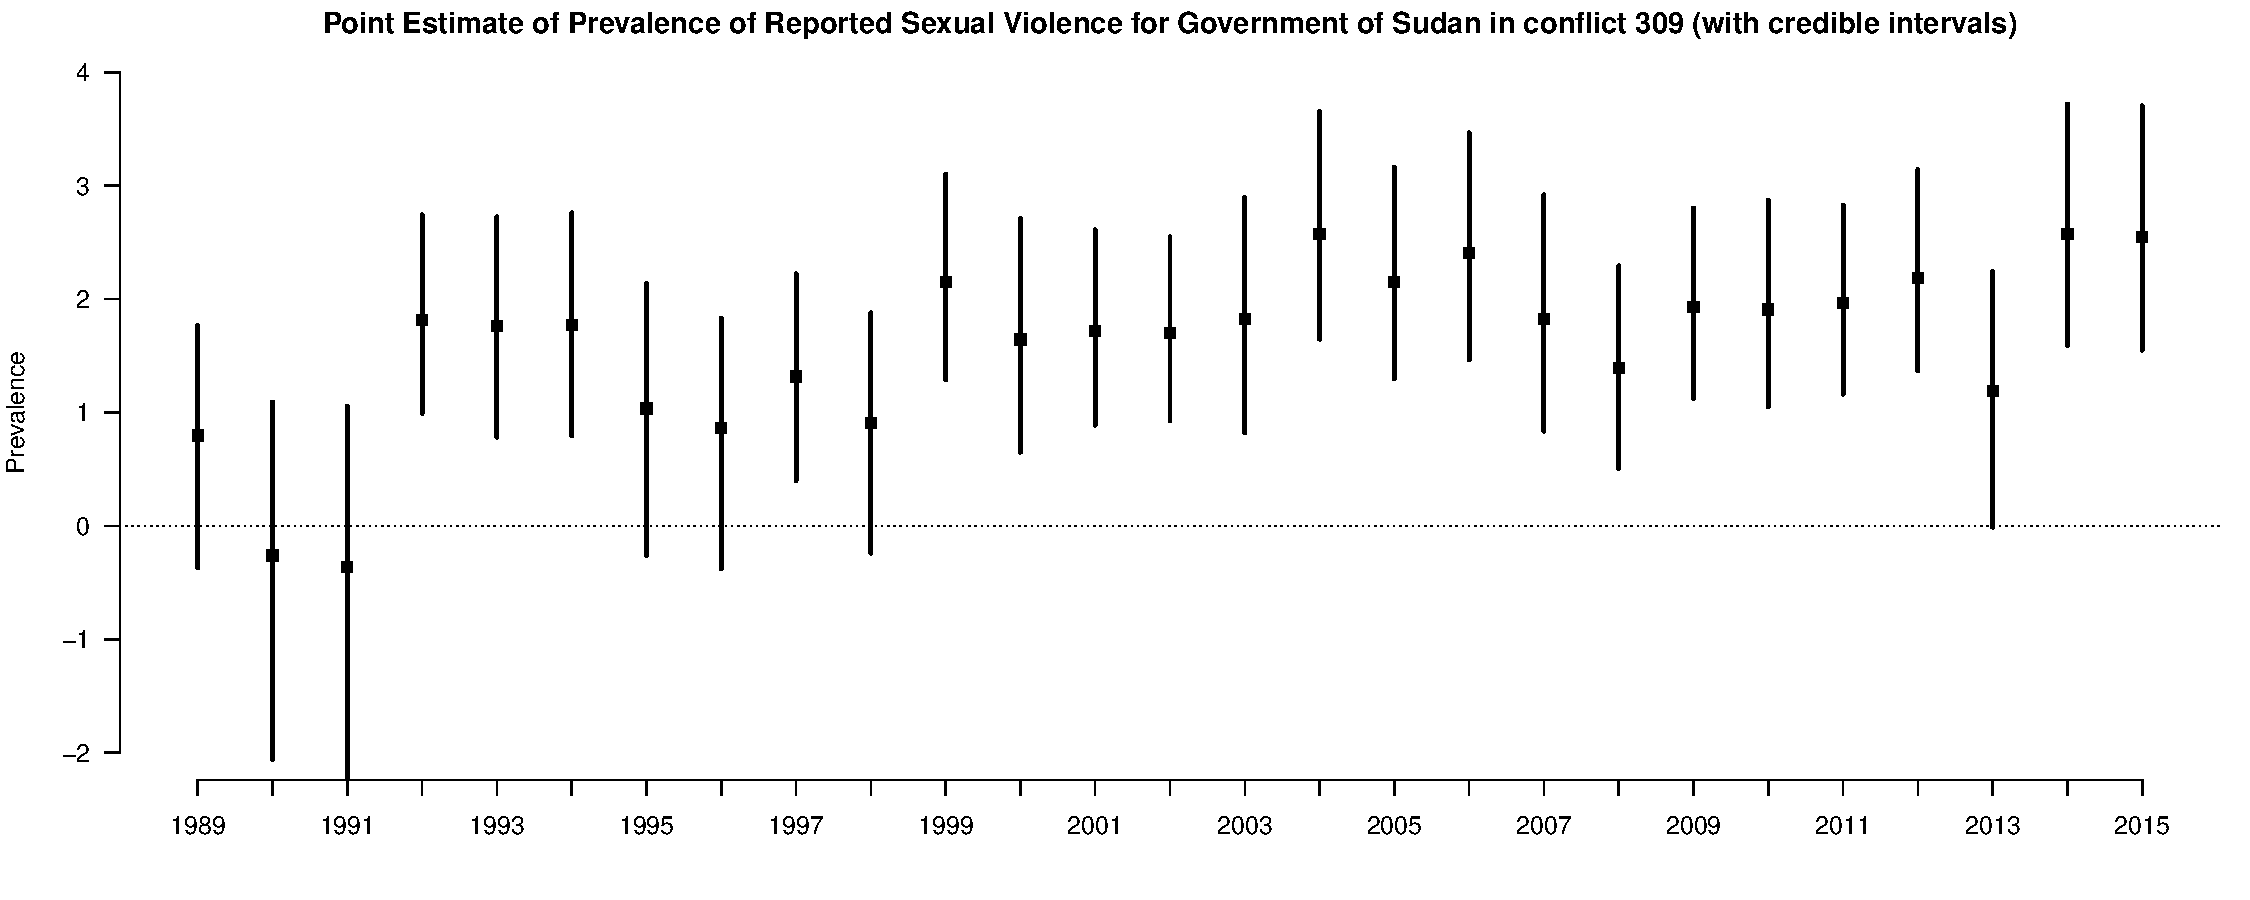
\includegraphics[width=11cm]{../visualize/output/pp-dynamic-estimates-Sudan-309.pdf}
\caption{Estimated level of engagement in wartime sexual violence by state forces in Sudan \hyperlink{SUDAN-static}{\beamerbutton{static}}}
\end{figure}
\end{frame}


\begin{frame}[label=DRC-dynamic]
\frametitle{Dynamic Estimates: DRC}
\begin{figure}\centering
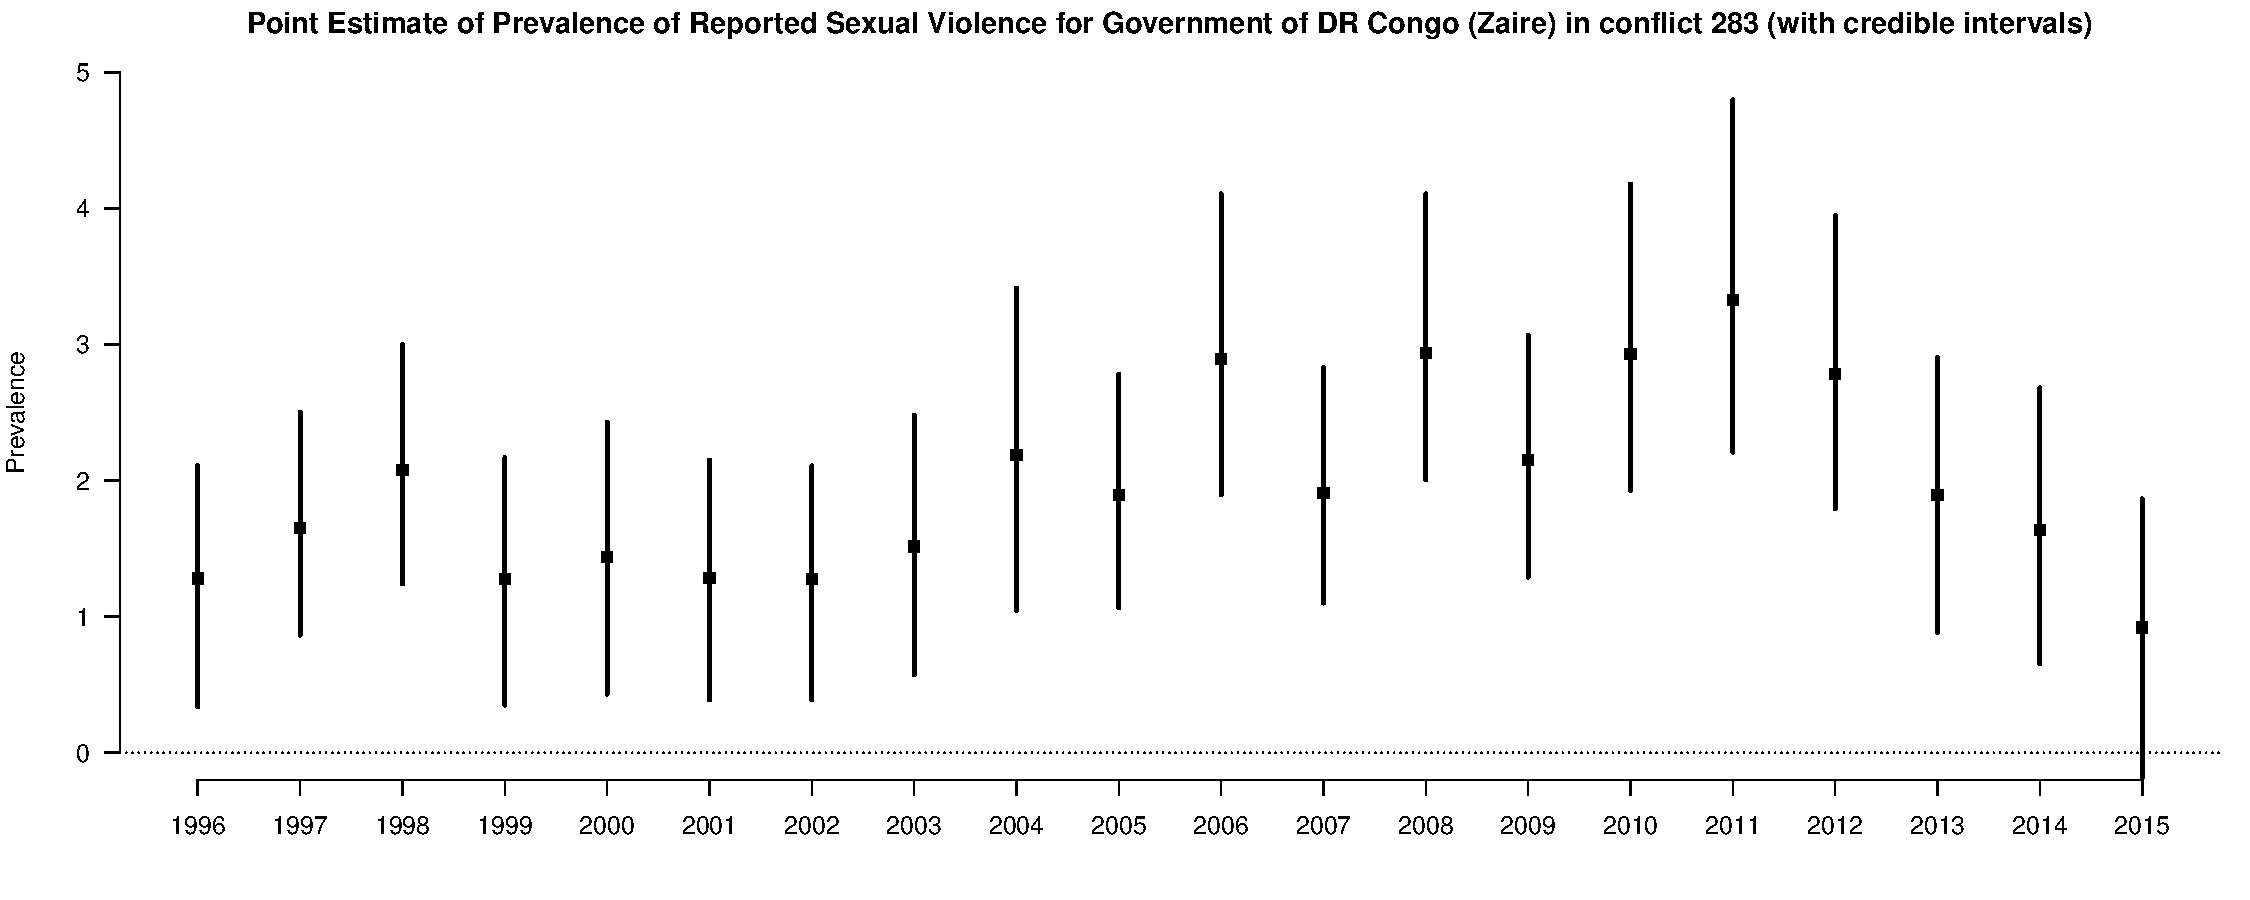
\includegraphics[width=11cm]{../visualize/output/pp-dynamic-estimates-DR-Congo-Zaire-283.pdf}
\caption{Estimated level of engagement in wartime sexual violence by state forces in DRC \hyperlink{DRC-static}{\beamerbutton{static}}}
\end{figure}
\end{frame}


\frame{\frametitle{Current State of this Research Project}

\begin{itemize}
\item Our goal is to develop a LVM approach for measuring wartime sexual violence. 

\item Currently, our main concern are the many conflict-years with zero observations, i.e., no reports of sexual violence.

\begin{itemize}
\item Did observational challenges impede our registration of sexual-violence conflict events?
\item Or, was there truly no conflict-related use of sexual violence?
\end{itemize}

\end{itemize}
}


\frame{\frametitle{Planned Next Steps}%\pause


\begin{itemize}
\item Include more indicators of wartime sexual violence 
\item Include measures of ``openness''/observability, such as freedom of press, local civil society, total number of sexual violence related news reports, etc.
\item Measure the level of event/actor/location (dis)agreement across human rights reports using text analysis
\item Explore the use of Bayesian Model Averaging to account for possible list dependence %%(e.g., sources drawing information from each other or relying on the same source material)
\item Conduct case studies to better understand data-generating processes and finetune models (e.g., Kashmir, Kosovo, ?)
\end{itemize}
}




\frame{
\centering
\LARGE{Thank you!}

\href{mailto:julianek@umich.edu}{Email me if you have questions or suggestions.}
}

\end{document}